\usetikzlibrary{calc}
% 2008安徽文科19四棱锥O-ABCD,M为OA中点
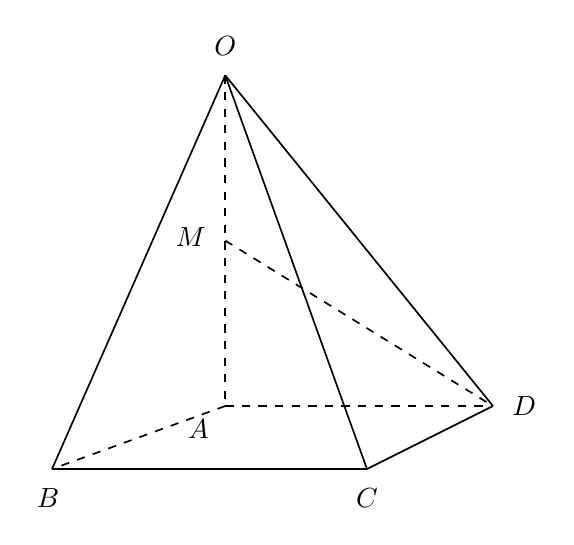
\begin{tikzpicture}[x=1cm,y=1cm,line width=0.6pt]
\coordinate (O) at (2.2,6.0);
\coordinate (M) at (2.2,3.9);
\coordinate (A) at (2.2,1.8);
\coordinate (B) at (0.0,1.0);
\coordinate (C) at (4.0,1.0);
\coordinate (D) at (5.6,1.8);
\draw[draw=black,dashed] (O)--(M)--(A);
\draw[draw=black,dashed] (A)--(B);
\draw[draw=black,dashed] (A)--(D);
\draw[draw=black,dashed] (M)--(D);
\draw[draw=black] (O)--(B);
\draw[draw=black] (O)--(C);
\draw[draw=black] (O)--(D);
\draw[draw=black] (B)--(C);
\draw[draw=black] (C)--(D);
\node[anchor=south,font=\normalsize] at ($(O)+(0,0.12)$) {$O$};
\node[anchor=east,font=\normalsize] at ($(M)+(-0.12,0.05)$) {$M$};
\node[anchor=north east,font=\normalsize] at ($(A)+(-0.08,-0.05)$) {$A$};
\node[anchor=north,font=\normalsize] at ($(B)+(-0.05,-0.12)$) {$B$};
\node[anchor=north,font=\normalsize] at ($(C)+(0,-0.12)$) {$C$};
\node[anchor=west,font=\normalsize] at ($(D)+(0.12,0)$) {$D$};
\end{tikzpicture}
